\chapter{Architecture Exploration}\label{models}
This chapter presents the proposed neural network architectures. It starts with a baseline TNN network implemented in \texttt{PyTorch}, which then undergoes a series of hardware-aware adaptions specific to jet tagging. During this process two separate architectures are developed, which differ by the input type and design goal. The first one, referred to as the \textit{ultra-low latency} one, targets the HLF jet representation and aims to achieve the lowest possible latency at the cost of accuracy and AUC values. The second one, called \textit{accuracy-focused}, is based on the constituent list jet representation and trade-offs latency for quality of classification while still remaining within L1T timing constraints.


\section{Base Architecture}
The starting point of this analysis is derived from transformer architecture used in the original paper \cite{44-vaswani2017attention} and recent proof-of-concept used for jet tagging \cite{3-yuan2021constituentnet:}. The overview of the network components can be seen in figure \ref{fig:constituent-net}.

\begin{figure}[hpt!]
  \centering
  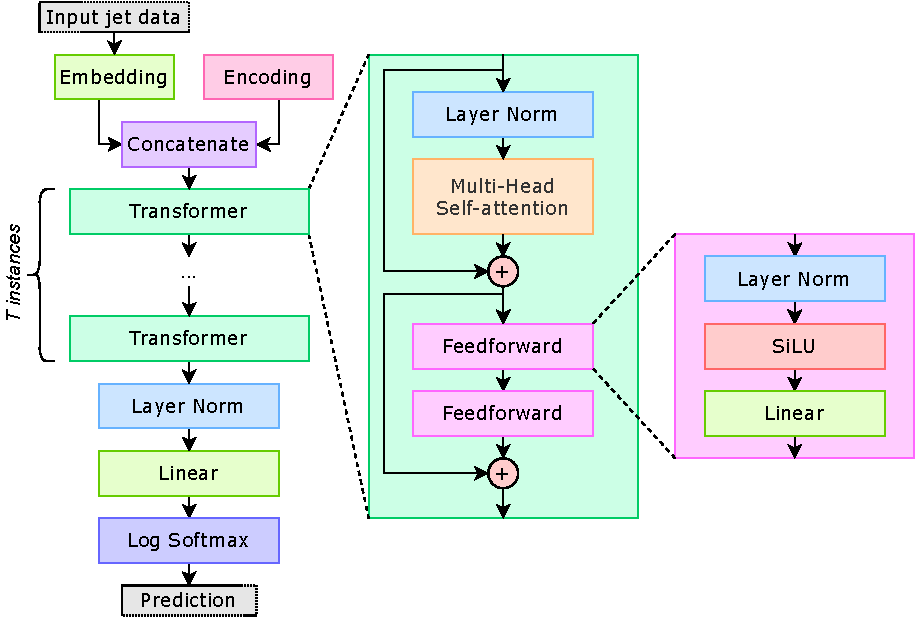
\includegraphics[trim={0cm 0cm 0cm 0cm}, width=0.6\textwidth, center]{models/constituent_net.pdf}
  \caption{Diagram with an overview of the baseline architecture.}
  \label{fig:constituent-net}
\end{figure}

The straight-forward path between model's input and output highlights the sequential nature of transformer which stands in opposition to recurrency present in GRU and LSTM models. While this allows for the aforementioned parallelizability and pipelining on FPGAs, it also poses a challenge of increased hardware footprint and synthesis complexity when compared to recurrent models, where the key components can get reused to meet the resource constraints. To better understand the transformer's complexity, the next subsections derive the equations linking the internal components and explain the involved terminology.


\subsection{Input embedding and Residual Connections}
Although the model lacks any recurrency, the transformer includes two residual connections which have been widely adopted since their successful application in ResNet neural networks \cite{75-kaiming2016deep}. They offer improvements to training time and resulting accuracy \cite{74-szegedy2016inception-v4}, however, they require standardized data dimensionality to ensure the summation can be logically executed. In this project, this is obtained thanks to input embedding, which transforms the input \(\bm{\hat{x^i}} \in \mathbb{R}^{L \times 16} \) into a shape \(\mathbb{R}^{L \times d}\) that is used through the design, as seen in equation \ref{eq:embedding}.

\begin{equation}\label{eq:embedding}
  \bm{\hat{x^i}_{\text{emb}}} = \text{embedding} ( \bm{\hat{x^i}} ) = w_{\text{embed}}\; \bm{\hat{x^i}} + b_{\text{embed}} \in \mathbb{R}^{L \times d}
\end{equation}

This dimensionality change can be conveniently performed using a linear layer, and it has to be remembered that each such layer increased the model learning capacity thanks to the learnable weights and bias. The network's inner dimension \(d\) is treated as a hyperparameter as it influences the model's accuracy and performance, but it has to be noted that the other dimension prevalent in the network comes from the input's number of jet constituents \(L\) (which is set to 1 in case of the HLS representation), meaning that the model is also susceptible to a parameter which cannot be easily tuned.


\subsection{Input Encoding}
Along the embedding, an input encoding is concatenated and fed to the transformer layer. In natural language processing, the encoding is meant to allow the model to benefit from the sequential information of the words in a sentence. It can be obtained from a sinusoidal function using the position index or simply treated as another learnable parameter. The sequential relations are not present in the jet data, because all the jets originate from the same proton-proton collision, hence, the latter approach is used in this project. It is worth mentioning, that from empirical analysis, the learnable encodings have a significant impact on the final results as they represent a trained, hidden state concatenated to all inputs during evaluation, as shown in equation \ref{eq:encoding}. Its impact is especially prevalent for the HLF data (where \(L = 1\)), where the hidden state matched input's dimension and effectively doubles it after concatenation.

\begin{equation}\label{eq:encoding}
  \text{encoding} ( \bm{\hat{x^i}_{\text{emb}}} ) = w_{\text{encoding}} \in \mathbb{R}^{1 \times d} \implies \text{concat} (\bm{\hat{x^i}_{\text{emb}}},\; w_{\text{encoding}}) \in \mathbb{R}^{(L+1) \times d}
\end{equation}

Choosing a learned hidden state is also more efficient for inference in hardware, as the increased training cost associated with back-propagation of this parameter yields a constant set of values that are known during compile-time of the FPGA and can be implemented using a LUT.


\subsection{Normalization and Parameter Extraction}
As layer normalization does not track and gather running mean and variance statistics, this mechanism is implemented on top of the existing \texttt{PyTorch} implementation to facilitate extracting the aggregated statistics after training. These, along with all the learned weights and biases, are extracted and transformed into specific C++ formats supported in HLS using a custom tool developed for this purpose. This allows for directly initializing the FPGA's BRAMs and LUTs with the model parameters, which avoids the need for an interaction with a host machine.

Obtaining the statistics taken for the data before normalization layers can also be viewed as a hardware-aware optimization. This can be explained with the mathematical derivation presented in equation \ref{eq:normalization-optimization}

\begin{equation}\label{eq:normalization-optimization}
  y = \frac{x - E[x]}{\sqrt{Var[x] + \epsilon}} \cdot \gamma + \beta = x \cdot (\frac{\gamma}{\sqrt{Var + \epsilon}}) + (\beta - \frac{\gamma * E}{\sqrt{Var + \epsilon}}) = w \cdot x + b
\end{equation}

By treating the mean \(E[x]\) and variance \(Var[x]\) of input \(x\) as learned parameters, the square root and division operations can be fully omitted by fusing them into the existing \(\gamma\) and \(\beta\) parameters which simplifies the hardware required for the normalization layers. This is especially useful as FPGAs lack dedicated hardware for these computationally expensive operations, which could lead to suboptimal designs being synthesized. Independently of the implementation in this work, a similar idea has been proposed and successfully used as an optimization in the past \cite{46-fan2018real-time}.

The algorithm behind the parameter extraction is rather simple, and the difficulty comes from the domain specific knowledge of handling \texttt{PyTorch} model parameters and generating the correct files for HLS. The break-down of the necessary steps can be seen in algorithm \ref{alg:parameter-extraction}.

\begin{algorithm}
  \caption{Mechanism behind model parameter extraction}\label{alg:parameter-extraction}
  \begin{algorithmic}[1]
    \State $state \gets $load\_state(model)
    \State sort($state$)
    \State $curr\_weight \gets $null
    \For{$param$ in $state$}
      \State $mean \gets $find\_mean(model, param)
      \State $var \gets $find\_var(model, param)

      \If{$param$ is weight}
        \State $curr\_weight \gets $param
        \State $new\_param \gets $update\_weight(param, var)

      \Else
        
        \State $new\_param \gets $update\_bias(param, curr\_weight, mean, var)
      \EndIf
      \State \texttt{save(new\_param)}
    \EndFor
  \end{algorithmic}
\end{algorithm}


\section{Hardware Mapping}


\subsection{Tensor Multiplication and Scaling}
Each self-attention head performs two tensor multiplications (referred to as \textit{matmul} blocks in figure \ref{fig:self-attention-multi-head}), which are normally expressed using Einstein Summation notation \cite{59-barr1991einstein}, which is supported by mathematical and machine learning libraries like \texttt{NumPy} or \texttt{PyTorch}. However, not present by default in HLS, it required careful design of the calculation loops in order to not cripple the performance by unnecessary computations and pseudo-random data accesses. As part of this research, an efficient and fully-customizable HLS block has been designed, that uses a very similar interface to the Python equivalent.

\begin{figure}[hpt!]
  \centering
  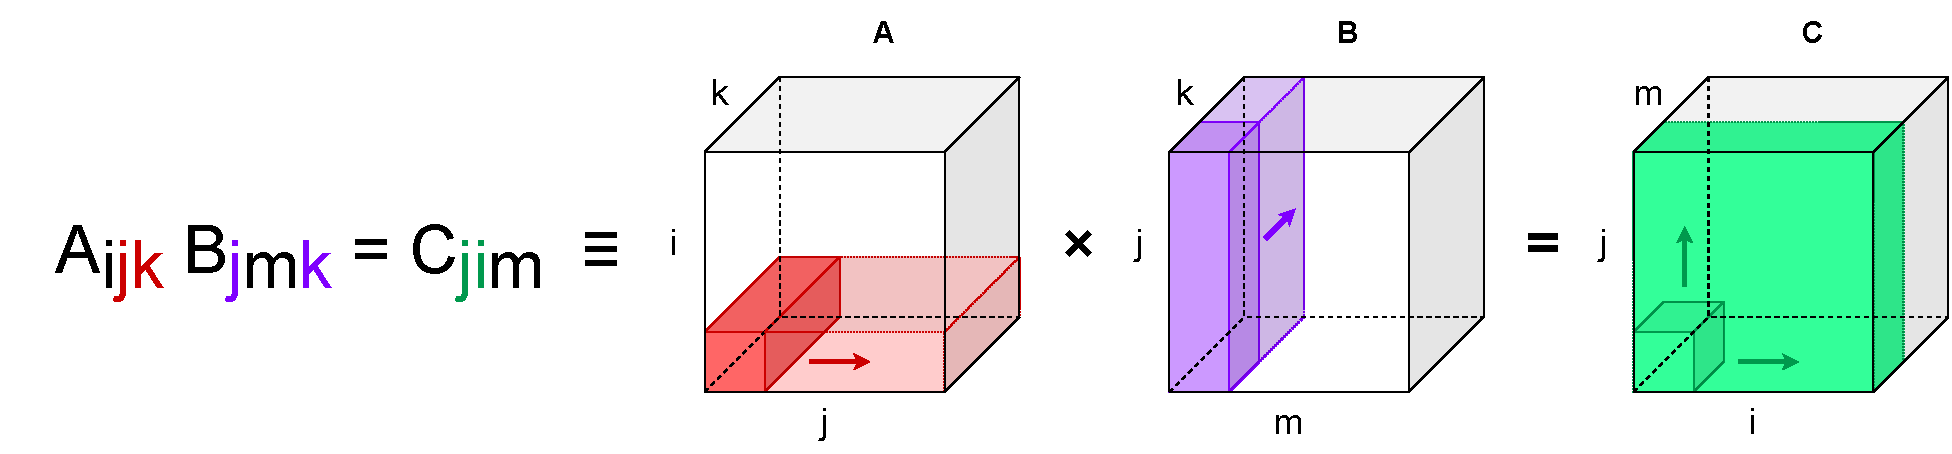
\includegraphics[trim={0cm 0cm 0cm 0cm}, width=0.8\textwidth, center]{models/einsum.pdf}
  \caption{Visualization of a tensor operation expressed in Einstein Summation notation.}
  \label{fig:einsum}
\end{figure}

Figure \ref{fig:einsum} shows a visualization for an example notation to give a better understanding of the necessary flexibility of a formula. The translation between notations using the custom tool is showcased in listing TODO. While the \texttt{PyTorch} implementation uses 4-dimensional tensors, the first dimension refers to the batch, which is not present in the hardware implementation that processes input samples one-by-one.

\todofig{Code listing showing starting \texttt{PyTorch} code and resulting C++ HLS implementation}
\todofig{|}
\todofig{|}
\todofig{|}
\todofig{|}
\todofig{|}

Another simple optimization used alongside the tensor multiplication blocks was the change in size scaling from using division to performing an arithmetic right shift (ASR), which requires precomputing the logarithm of the size, seen in equation \ref{eq:log-div}, vastly simplifying the otherwise computationally expensive hardware required at run-time.

\begin{equation}\label{eq:log-div}
  \frac{x}{\sqrt{\text{size}}} \equiv \text{ASR}(x,\; \log_2 \sqrt{\text{size}}) \equiv \text{ASR}(x,\; \frac{1}{2}\log_2 \text{size})
\end{equation}


\subsection{Softmax and Log Softmax Activation}
Despite an already existing \hlsml implementation of the softmax activation function, computing the logarithm of its result is not as simple as it may seem. This is because the numerical stability and computational efficiency of this operation is often explored in-depth \cite{60-blanchard2019accurate} and varies depending on the programming language and target platform.

\begin{figure}[hpt!]
  \centering
  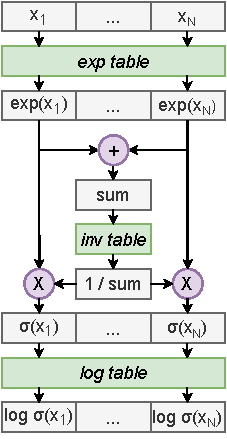
\includegraphics[trim={0cm 0cm 0cm 0cm}, width=0.2\textwidth, center]{models/log_softmax_naive.pdf}
  \caption{Direct hardware implementations of log softmax.}
  \label{fig:log-softmax-naive}
\end{figure}

The naive implementation comes straight from the definition of taking a logarithm of softmax, seen in equation \ref{eq:softmax}, and the required hardware operations are shown in figure \ref{fig:log-softmax-naive}.

\begin{equation} \label{eq:softmax}
    \sigma (x_i) = e^{x_i} / \sum_{j=1}^{N} e^{x_j}
\end{equation}

This report proposes a different way of mapping this operation to hardware to improve stability while shortening the critical path and using less resources. It is based on the derivation shown in equation \ref{eq:log-softmax}.

\begin{equation} \label{eq:log-softmax}
    \log (\sigma (x_i)) = log(e^{x_i} / \sum_{j=1}^{N} e^{x_j}) = \log(e^{x_i}) - \log(\sum_{j=1}^{N} e^{x_j}) = e^{x_i} - \log(\sum_{j=1}^{N} e^{x_j})
\end{equation}

The resulting hardware operations are depicted in figure \ref{fig:log-softmax-opt}. It is important to note, that operations like exponentiation, division or taking a logarithm usually rely on precomputing a wide range of values and mapping them in BRAMs or LUTs to allow for lookup on run-time. Hence, the optimized design requires one less of such lookups while also replacing multiplication by a subtraction, which can be simpler to express in hardware.

\begin{figure}[hpt!]
  \centering
  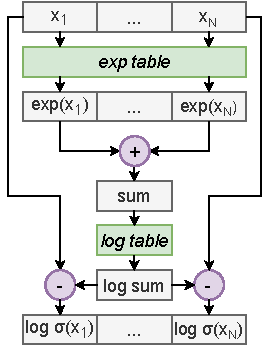
\includegraphics[trim={0cm 0cm 0cm 0cm}, width=0.2\textwidth, center]{models/log_softmax_opt.pdf}
  \caption{Optimized hardware implementations of log softmax.}
  \label{fig:log-softmax-opt}
\end{figure}

Although further simplifications, including approximating the summation by finding the maximum (see equation \ref{eq:log-softmax-max}) or simply omitting the logarithm portion of the expression, were also explored, they noticeably lowered the final accuracy and were thus abandoned.

\begin{equation} \label{eq:log-softmax-max}
    \log (\sigma (x_i)) = e^{x_i} - \log(\sum_{j=1}^{N} e^{x_j}) = e^{x_i} - \sum_{j=1}^{N} \log(e^{x_j}) = e^{x_i} - \sum_{j=1}^{N} x_j \approx e^{x_i} - \max(x)
\end{equation}


\section{Ultra-Low Latency Architecture}

\subsection{Simplification and Tuning}

\subsection{Hardware Mapping}


\section{Accuracy-Focused Architecture}
\indo{stability issues solved by more normalization (coming from wide range of inputs of 30x16)}

\subsection{Hardware Mapping}

